\documentclass[conference]{IEEEtran}
\IEEEoverridecommandlockouts
% The preceding line is only needed to identify funding in the first footnote. If that is unneeded, please comment it out.
\usepackage{hyperref}
\usepackage{cite}
\usepackage{amsmath,amssymb,amsfonts}
\usepackage{algorithmic}
\usepackage{graphicx}
\usepackage{textcomp}
\usepackage{xcolor}
\def\BibTeX{{\rm B\kern-.05em{\sc i\kern-.025em b}\kern-.08em
    T\kern-.1667em\lower.7ex\hbox{E}\kern-.125emX}}
\begin{document}

\title{Classification of cognitive workload reliability considering easy and complex mathematical tasks\\}


\author{\IEEEauthorblockN{\textsuperscript{} Marco Minchella}
\IEEEauthorblockA{\textit{Department of information engineering} \\
\textit{Università degli studi di Padova}\\
Padova, Italy \\
marco.minchella@studenti.unipd.it}
\and
\IEEEauthorblockN{\textsuperscript{} Martina Canini}
\IEEEauthorblockA{\textit{Department of information engineering} \\
\textit{Università degli studi di Padova}\\
Padova, Italy \\
martina.canini@studenti.unipd.it}

}

\maketitle

\begin{abstract}
This study explored the feasibility of using in-ear EEG for classifying cognitive workload.  The research utilized a dataset acquired by IDUN Technologies involving a single participant engaged in three phases of mathematical tasks with varying difficulty levels, while wearing an in-ear EEG device.  A range of signal processing techniques and feature extraction methodologies were applied, including Welch's method for power spectral density estimation, to analyze the EEG data. Feature vectors were then constructed from each data segment, encompassing statistical, temporal, and frequency domain features.  These feature vectors were then used to train various machine learning classifiers, including a Random Forest, Perceptron, and Support Vector Machine (SVM), to discriminate between different cognitive workload levels. Notably, the study investigated the effectiveness of feature selection methods, such as SelectKBest, in reducing the dimensionality of the feature space and potentially improving classifier performance. The results indicated that in-ear EEG recordings, combined with appropriate feature selection and machine learning models, can effectively differentiate between distinct cognitive workload levels.  The study emphasizes the potential of in-ear EEG as a cost-effective and comfortable alternative to traditional EEG for evaluating cognitive workload, a key factor in various fields such as human-computer interaction, neuroergonomics, and cognitive science. 
\end{abstract}

\begin{IEEEkeywords}
EEG, BCI,in-ear-EEG, Data reliability, Machine Learning 
\end{IEEEkeywords}

\vspace{2mm}
\section{Introduction}
\vspace{2mm}

The intrinsic electrical activity of the brain is captured through electroencephalography (EEG), a phenomenon which arises from the movement of ionic currents across neuronal membranes, a byproduct of the information processing performed by neurons in the human brain, which generates electric and magnetic fields. These electrical fields are detected by affixing electrodes to the scalp's surface. 

EEG offers several advantages over alternative brain function assessment techniques, such as reduced hardware costs and the elimination of exposure to radiation or the need for injections, making it an exceptionally safe investigation modality. Furthermore, EEG provides superior temporal resolution, being capable of capturing changes on the millisecond scale as opposed to seconds. 

The EEG signal is subdivided into distinct frequency bands: delta (0.5–4 Hz), theta (4–7.5 Hz), alpha (7.5–14 Hz), beta (14–40 Hz), and gamma (above 40 Hz). These frequency bands are indicative of various cognitive states, and deviations from normative EEG patterns can assist clinicians in diagnosing neurological disorders\cite{7813897}.

The inherent discomfort of traditional EEG systems: scalp-EEG, has motivated the development of in-ear EEG devices. These devices, designed to capturing neural signals via electrodes positioned within the ear canal, offer a promising avenue for advancing Brain-Computer Interfaces (BCI) by enhancing user comfort and promoting widespread adoption\cite{7858176}. 

\vspace{2mm}
\section{Materials and Methods}
\vspace{2mm}

\subsection{Data recording and experiment} 
\label{sec:DRaE}

We analyzed a dataset from a study executed by IDUN Technologies, where only the ear-centric EEG signal was acquired. The investigation involved a single participant engaged in solving mathematical tasks while equipped with the IDUN Guardian earbud, a single-channel EEG apparatus with the reference electrode situated in the left ear canal. The experimental protocol was segmented into three phases: an initial series of simple arithmetic tasks, followed by more challenging problems, and concluding with another sequence of simple tasks.

The EEG data for the cognitive workload assessment were recorded over a duration of approximately 7 minutes at a sampling rate of 250 Hz.

%-----Dataset-----

\vspace{2mm}
\section{Dataset}
\vspace{2mm}

\subsection{Raw signal and preprocessing}

The employed dataset comprised both unprocessed (raw) and preprocessed (filtered) signals. Typically, the raw signal would undergo processing through a filter bank to eliminate artifacts like line noise, followed by various procedures such as Independent Component Analysis (ICA). 

However, for this study, it was chosen to employ the already preprocessed signal. Given that the preprocessing was conducted by IDUN Technologies, we determined that this represented the optimal filtering approach available, and any additional attempts at processing on our part would likely have been inferior.

The entire filtered EEG recording is plotted in Fig. \ref{fig:EEG_data}.

\begin{figure}[htbp]
\centerline{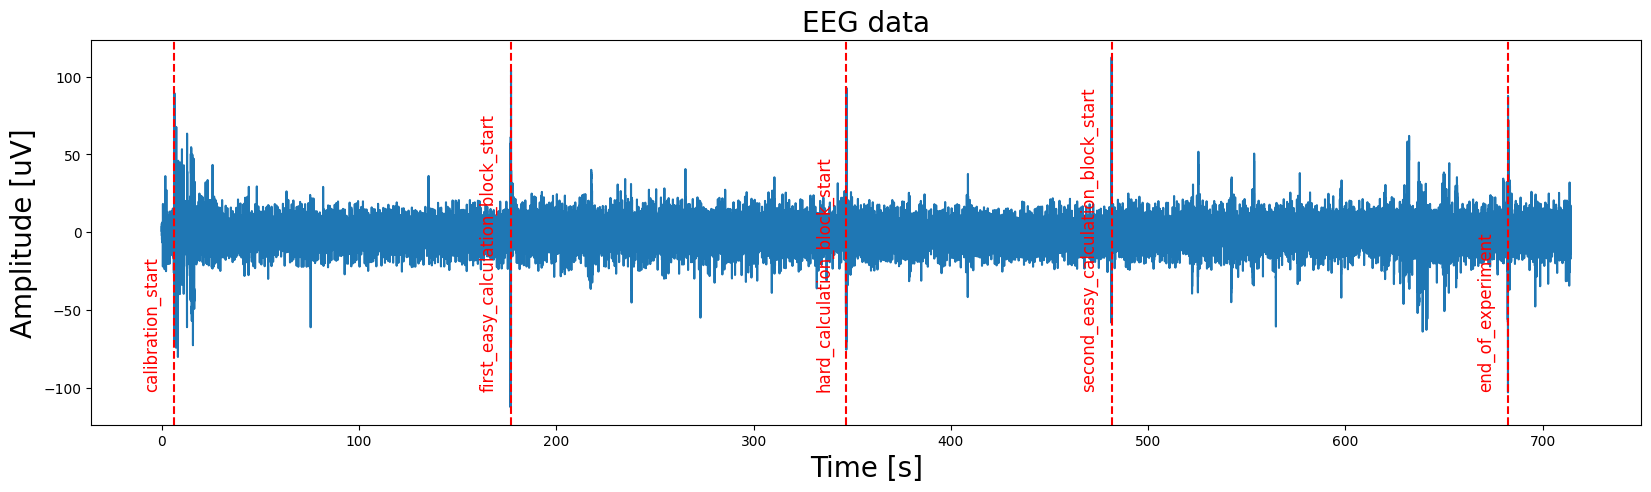
\includegraphics[scale=0.16]{Immagini E Health 2/eeg_data.png}}
\caption{Filtered EEG recording of the entire experiment.}
\label{fig:EEG_data}
\end{figure}

\subsection{Data and data cleaning}
\label{sec:Ddc}

The pre-processed dataset was provided in a Comma-Separated Value (CSV) format, with each sample containing a timestamp, EEG value, and label. The label field indicated one of five distinct conditions: calibration, initial easy calculation phase, challenging calculation phase, second easy calculation phase, and end of experiment. For the purpose of this analysis, the timestamp field was removed from each sample, and all samples labeled as calibration or end of experiment were discarded as they provided negligible information relevant to the classification problem. 

To visually explore potential features within the frequency domain, PSD plots were generated for the three aforementioned experimental sections. As expected, discerning salient characteristics in the frequency domain through visual inspection proved challenging, however, a subtle similarity between the PSD plots of the two easy calculation phases was observed.

To compute the spectral density of the signals across the three tasks, we initially computed the Fast Fourier Transform (FFT) on all samples within each dataset. As stated in  sec. \ref{sec:DRaE}, the EEG recording lasts about 7 minutes and is recorded with a 250 Hz sampling rate.

To assess the PSD the datasets has been devided into distinct segments and it was applied the Welch algorithm to further refine our analysis.

Welch's method enhances PSD estimation by segmenting the input signal into overlapping parts, each subjected to a window function to reduce spectral leakage. For each windowed segment, the FFT is computed. The periodogram, obtained by squaring the normalized FFT magnitude, is averaged across segments for the PSD estimate.

This averaging reduces variance compared to single-periodogram methods. The PSD is mathematically expressed as:

\[
P(f) = \frac{1}{KU} \sum_{k=1}^{K} \left| \sum_{n=0}^{L-1} x_k[n] w[n] e^{-j2\pi fn/N} \right|^2 
\]

Welch's technique balances frequency resolution and variance, making it widely used in applications like EEG analysis, as suggested by Art. \cite{Goker2023-tq}, to identify frequency components related to cognitive states.

Fig. \ref{figPSD1}, \ref{figPSD2}, and \ref{figPSD3} depict the Power Spectral Density (PSD) of the EEG signal during the three distinct phases of the experiment. 

Fig. \ref{figPSD1} represents the PSD during the initial phase, characterized by simple computational tasks. Fig. \ref{figPSD2} displays the PSD during the second phase, involving more challenging computations. Finally, Fig. \ref{figPSD3} illustrates the PSD during the third phase, where the participant again engaged in simple computational tasks. 
For the computation of the PSD of the EEG signal by Welch’s method, the latter has been segmented with a 500-sample Hanning window, overlapping by 250 samples, and 1024 points have been used for fine FFT frequency resolution.

\begin{figure}[htbp]
\centerline{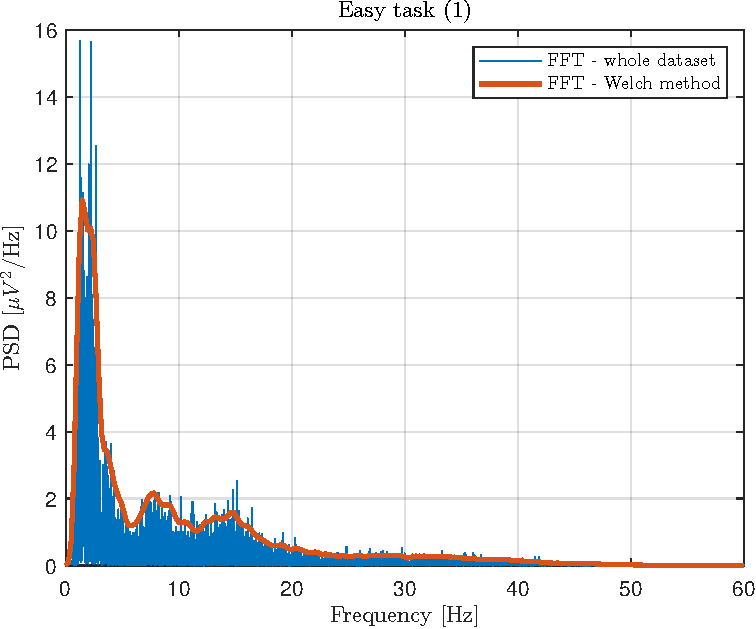
\includegraphics[scale=0.6]{EH_FFTEasy1.pdf}}
\caption{PSD of EEG during first task.}
\label{figPSD1}
\end{figure}

\begin{figure}[htbp]
\centerline{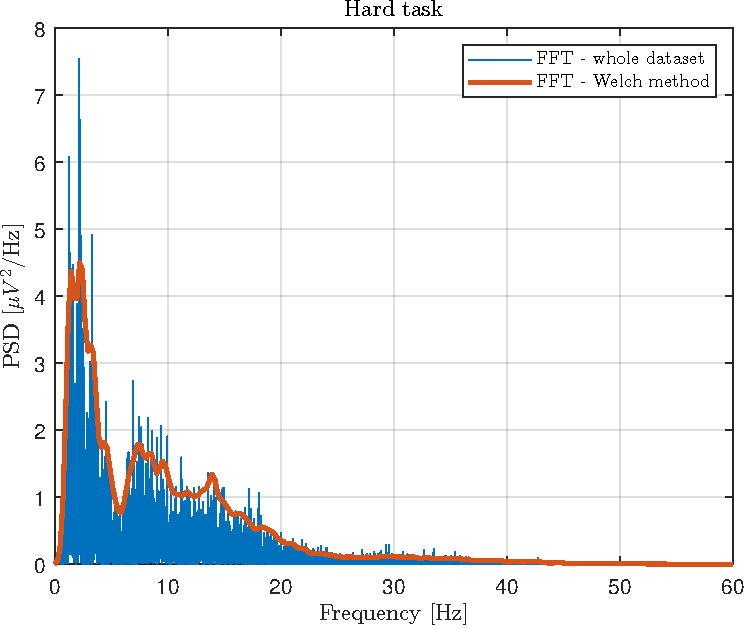
\includegraphics[scale=0.6]{EH_FFTHard2.pdf}}
\caption{PSD of EEG during second task.}
\label{figPSD2}
\end{figure}

\begin{figure}[htbp]
\centerline{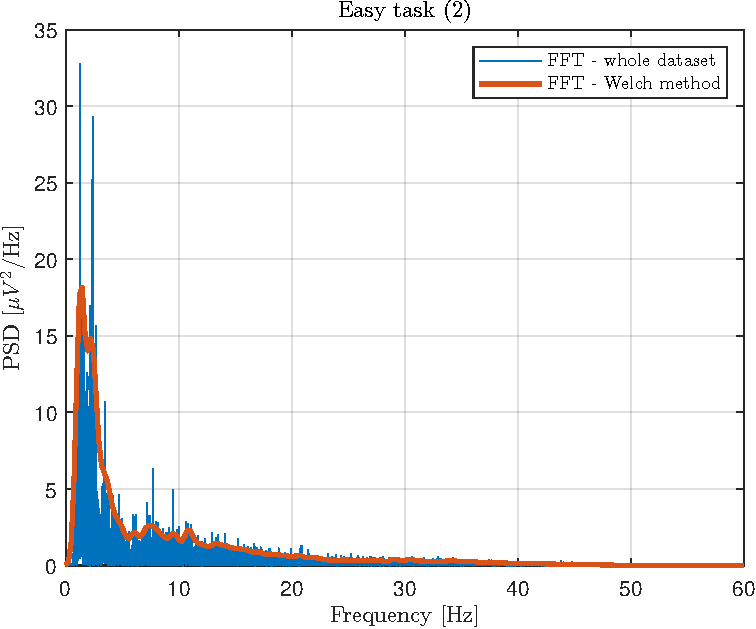
\includegraphics[scale=0.6]{EH_FFTEasy3.pdf}}
\caption{PSD of EEG during third task.}
\label{figPSD3}
\end{figure}



%-----Datapoints-----
\newpage
\subsection{Datapoints}

To prepare the data for classification, each of the three experimental recordings was segmented into 1-second epochs and any residual sample that did not align with the epoch length was discarded. This segmentation process facilitated the extraction and selection of features from each data point, enabling the classification of each segment as representing either ``easy" or ``hard" computational tasks. 

A notable challenge encountered in this dataset was the class imbalance: there were 370 data points labeled as ``easy" and only 134 labeled as ``hard." This disparity raised concerns about potential bias in the training dataset, potentially leading to a model that is disproportionately influenced by the more abundant class.

%-----Feature Extraction-----

\vspace{2mm}
\section{Feature Extraction}
\vspace{2mm}

Feature extraction was performed on each datapoint, encompassing both temporal and frequency domain features.

\subsection{Time features}
\label{AA}

Employing the SciPy and NumPy libraries, we extracted the following temporal domain features:
\begin{itemize}
    \item Mean
    \item Variance
    \item Standard deviation
    \item Peak to peak
    \item Minimum value
    \item Maximum value
    \item Index of minimum value
    \item Index of maximum value
    \item Mean square
    \item Root mean square
    \item Absolute discrete difference between adjecent datapoints
    \item Skewness
    \item Kurtosis
\end{itemize}

\subsection{Frequency features} \label{subsec:Ff}

Frequency domain features were computed, encompassing the power within the delta (0.5–4 Hz), theta (4–8 Hz), alpha (8–12 Hz), beta (12–30 Hz), and gamma (30–80 Hz) frequency bands. The bandpower function within MATLAB was utilized to calculate these features and subsequently, the data was transferred back to Google Colaboratory for further analysis.
\vspace{2mm}
\section{Classifiers and respective Results}
\vspace{2mm}
Several machine learning classifiers were employed to differentiate between task conditions based on all extracted features, after this step we proceeded to reduce the feature space by performing feature selection.

\subsection{Perceptron model}

The Perceptron model, a simple linear classifier, effectively identified linear decision boundaries, but its performance was somewhat limited due to the complexity of EEG signals, as illustrated in the confusion matrix presented in Fig. \ref{figcmP}. Nonetheless, it served as a useful baseline, allowing for comparison with more sophisticated techniques.
The training loss for the perceptron was 0.09 and the test loss was 0.14.

\begin{figure}[htbp]
\centerline{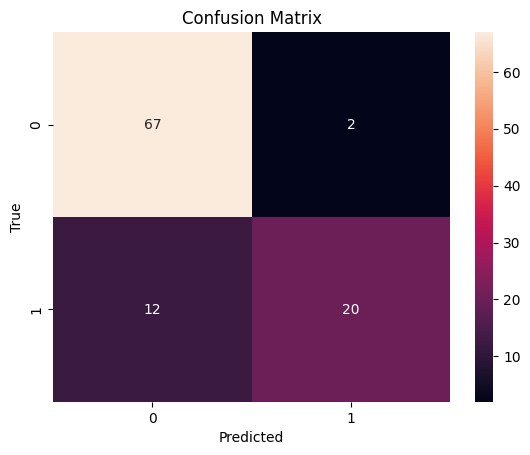
\includegraphics[scale=0.45]{binary_classification_perceptron.png}}
\caption{Confusion Matrix of binary classification using the perceptron method.}
\label{figcmP}
\end{figure}

\subsection{Random Forest Classifier}

The Random Forest Classifier offered a robust predictive performance with an accuracy that highlighted its ability to handle the complexity and variability in EEG data. This classifier's ensemble approach, which combines the predictions of multiple decision trees, proved effective in capturing nonlinear relationships within the data, offering flexibility and improved generalization over single models such as decision trees. The random forest model achieved notable accuracy in identifying task conditions, underscoring its suitability for EEG-based cognitive load classification.
The training loss for the RFC was 0 and the test loss was 0.04.

\subsection{Support Vector Machine}

The Support Vector Machine (SVM), particularly with a linear kernel, was explored due to its effectiveness in high-dimensional spaces like those formed by EEG features. SVM excelled in binary classification tasks where the classes are somewhat separable and provided high accuracy by maximizing the margin between the two classes, as evidenced by the confusion matrix depicted in Fig. \ref{figcmRF}. However, this technique's performance can be sensitive to the choice of kernel and parameters, indicating the need for careful tuning.
The training loss for the SVM was 0.04 and the test loss was 0.05.

\begin{figure}[htbp]
\centerline{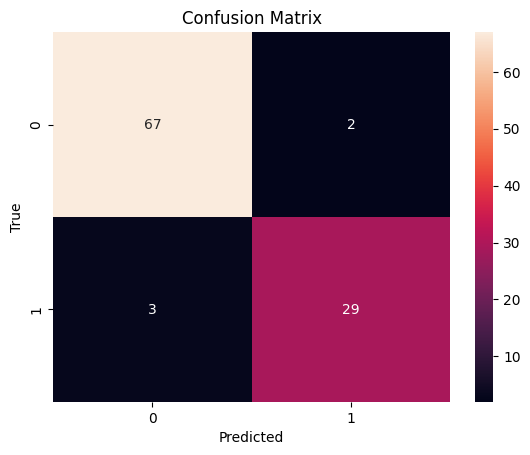
\includegraphics[scale=0.45]{ConfusionSVM.png}}
\caption{Confusion Matrix of binary classification using the SVM with linear kernel.}
\label{figcmRF}
\end{figure}


\vspace{2mm}
\section{Feature selection}
\vspace{2mm}

To potentially enhance model efficiency and improve performance, a feature selection process was implemented to reduce the dimensionality of the feature space. Subsequent to this, a second round of classification was conducted using SVM to assess any improvements in the results.

\subsection{Powerbands only method}

The initial approach involved manually selecting features, specifically excluding all temporal features and retaining only the powerband values. This selection was predicated on the premise that distinct states of cerebral activity exhibit unique values within the five previously described powerbands (subsection \ref{subsec:Ff}). The outcomes achieved using this method were suboptimal, with a training loss of 0.12 and a test loss of 0.14. These values are notably higher than those obtained without any form of feature selection.

\subsection{\texttt{SelectKBest} method}

To refine the feature set and enhance classification efficiency, the \texttt{SelectKBest} method was employed, automatically selecting the most discriminative features based on the mutual information criterion. This approach focused on identifying the most significant features, effectively reducing computational complexity and improving model performance without compromising accuracy.  Setting k=5 resulted in the selection of the following features: mean, index of minimum value, mean square, root mean square, and beta power band. Both the training and test losses exhibited promising results, with values of 0.05 and 0.08, respectively, indicating superior performance compared to utilizing solely power band features.

\subsection{Augmented SelectKBest method}

To enhance the performance of the \texttt{SelectKBest} feature selection process, the alpha and theta powerbands were incorporated into the feature space. This decision was informed by prior research on cognitive workload, which demonstrated that the theta powerband serves as a robust indicator of cognitive workload, with alpha and beta powerbands also exhibiting significant influence \cite{chikhi2022eeg}.  Augmenting the feature space with this strategy yielded a notable improvement, with the training loss decreasing to 0.06 and the test loss to 0.04.

\begin{figure}[htbp]
\centerline{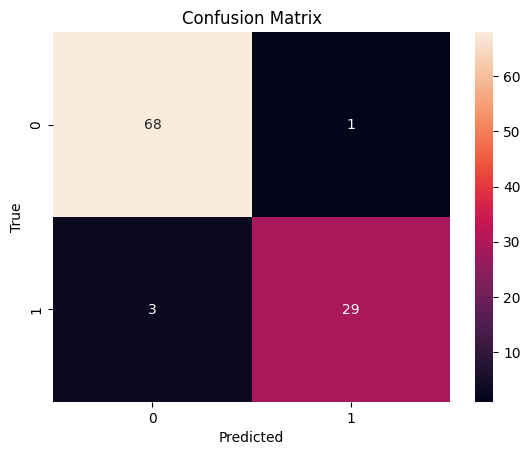
\includegraphics[scale=0.45]{ConfusionAug.png}}
\caption{Confusion Matrix of binary classification using SVM and augmanted \texttt{SelectKBest} feature selection method.}
\label{figcmMRF}
\end{figure}

\section{Multiclass classification}

To investigate potential changes in cerebral activity associated with habituation to mathematical tasks or increased relaxation over the course of the experiment, a multi-class classification was conducted using the Random Forest algorithm. This involved distinguishing not only between hard and easy tasks but also between the two distinct easy task phases. However, the classifier consistently failed to differentiate between the first and second easy tasks, both with and without the augmented SelectKBest strategy. This limitation is clearly evident when examining the confusion matrices depicted in Figures \ref{CnfMulti1} and \ref{CnfMulti2}.

\begin{figure}[htbp]
\centerline{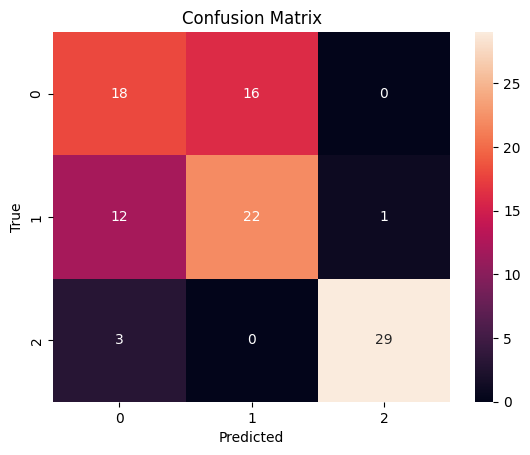
\includegraphics[scale=0.45]{multiclass_random_forest.png}}
\caption{Confusion Matrix of multiclass classification using Random Forest method without feature selection.}
\label{CnfMulti1}
\end{figure}

\begin{figure}[htbp]
\centerline{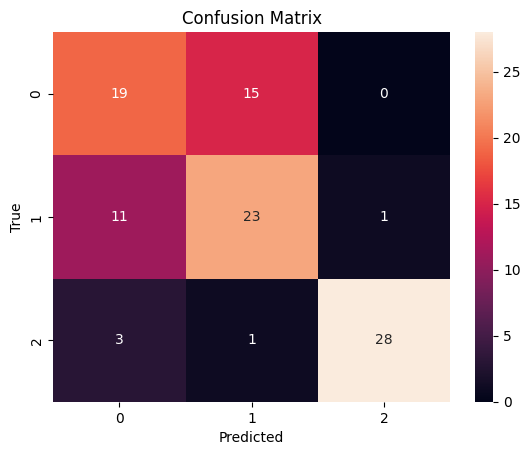
\includegraphics[scale=0.45]{COnfusion3Aug.png}}
\caption{Confusion Matrix of multiclass classification using Random Forest method with feature selection.}
\label{CnfMulti2}
\end{figure}

\newpage
\vspace{2mm}
\section{Conclusions}
\vspace{2mm}

The study showed how combining statistical, temporal, and frequency domain features from EEG data allows for a robust classification of cognitive load levels. Machine learning models effectively separated the conditions, with feature selection critically enhancing model performance.

The results of this investigation highlight the significant potential of ear-EEG-based classification for cognitive tasks, demonstrating its viability for practical BCI applications. This finding aligns with prior research, as reported in Art. \cite{Kaongoen_2023}, which underscores the remarkable potential of in-ear-EEG data for clinical monitoring.  This technology positions itself as a valuable resource for researchers, clinicians, and engineers actively contributing to the field of neural engineering

As a continuation of the current investigation, the methodologies outlined herein could be applied to the raw signal without any supplementary filtering. The resulting outcomes could then be juxtaposed with those obtained from the present analysis, aiming to identify concordant findings. Should similar results be observed, this would prove beneficial, as it could potentially eliminate the initial signal pre-processing phase. 

Additionally, further exploration of diverse deep neural network architectures could yield valuable insights such as in the work by \cite{9061644}. The objective would be to identify the minimal complexity solution capable of generating predictions with sufficient accuracy.

%-----Code-----

\vspace{2mm}
\section{Code}
\vspace{2mm}

The compiled Python Colab code for this study can be found at:
\url{https://colab.research.google.com/drive/1AiCC8l1vArFH3wiKJTHVzw1a2ZsXBbQM?usp=sharing}.

%-----References-----

\bibliographystyle{plain}
\bibliography{references} % Entries are in the refs.bib file

\end{document}
